%\labsec{results}
%-------------------------------------------------------------------------------------------------------------------------
\subsection{Simple Simulations}
%-------------------------------------------------------------------------------------------------------------------------



\begin{figure}[H]
	\centering
	\begin{subfigure}{0.85\textwidth}
		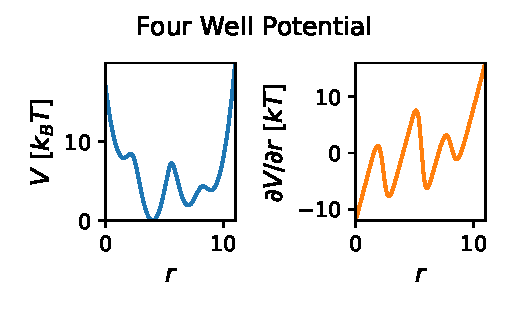
\includegraphics[width=\linewidth, height=1.75in]{fig/codeExamples/four_well.pdf} 
		\caption{}
	\end{subfigure}\\
	\begin{subfigure}{0.85\textwidth}
		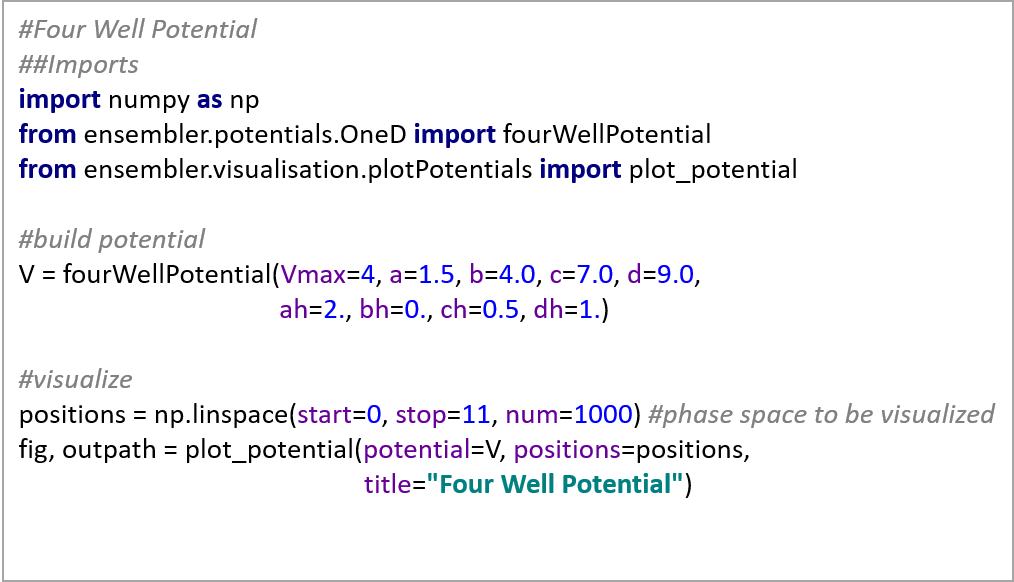
\includegraphics[width=\linewidth, height=1.75in]{fig/codeExamples/Potential_code.png}
		\caption{}
	\end{subfigure}
	\caption{A four-well potential-energy surface visualized by the standard visualization function of Ensembler. (a) Potential-energy function (blue) and the automatically generated spatial gradient (orange) over a given coordinate range. (b) Source code to define the potential-energy function and the coordinate range to be visualized. These parameters are passed to the built-in plotting function in the \textit{potential classes} of Ensembler.}
	\label{fig:code_example_potential}
\end{figure}



In the following, simple code examples are shown to introduce the usage of Ensembler. In addition, an application example is provided to illustrate the use of Ensembler for teaching about free-energy methods. 
The code for these examples can be found in the GitHub repository \textit{\hyperlink{https://github.com/rinikerlab/Ensembler}{https://github.com/rinikerlab/Ensembler/examples}}.


In typical applications of Ensembler, the user selects a potential-energy function from the available ones. In the following example, a potential-energy function with four wells is selected and initialized with chosen parameters. 
To sample this four-well potential-energy function with stochastic dynamics (SD),\cite{Brunger1984} the sampling method is instantiated and passed to the \textit{system class}, which controls the execution of the simulation. 
The simulation is performed by calling the function \textit{simulate} with the desired number of simulation steps passed as parameter. 
Subsequently, the results can be visualized using the built-in visualization functions that are compatible with the \textit{simulation class} of Ensembler.  
As can be seen in Figure \ref{fig:code_example_simulations}a, the energy barriers between the different minima were not crossed during the chosen simulation length. 
To overcome the sampling issue, enhanced sampling techniques can be employed.\cite{Pohorille2010} 
In this example, local elevation\cite{Huber1994}/metadynamics\cite{Laio2002} is used to overcome the energy barriers (Figure \ref{fig:code_example_simulations}b).
The method adds a time-dependent biasing potential to the system, i.e. it adds a Gaussian biasing potential to positions that were already visited such that they become energetically less favorable. This decreases the likelihood of visiting known positions again. 
The enhanced sampling technique can be applied by adding a single line of code compared to the previous simulation (Figure \ref{fig:code_example_simulations}c).

\begin{figure}[H]
	\centering
	\begin{subfigure}{\textwidth}
		\caption{Standard Langevin Simulation}
		\centering
		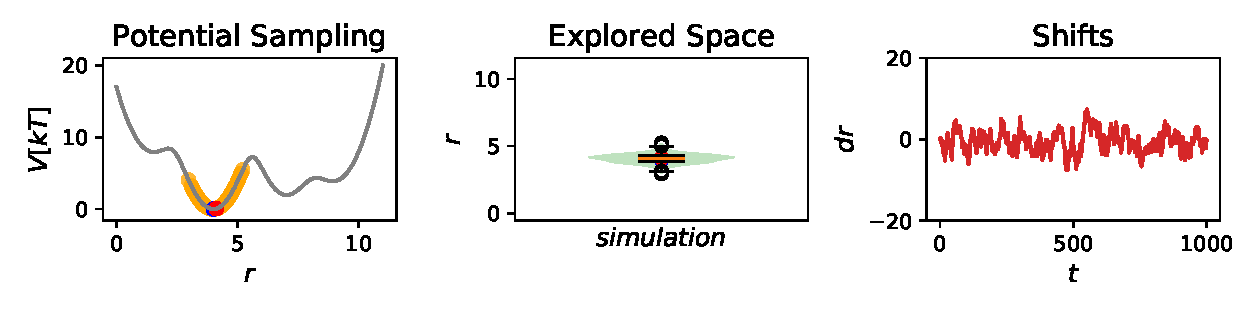
\includegraphics[width=0.85\linewidth]{fig/codeExamples/langevin_simulation.pdf} 
	\end{subfigure}
	\vspace{2.5mm}
	\begin{subfigure}{\textwidth}
		\caption{Langevin Simulation with Local Elevation/Metadynamics}
		\centering
		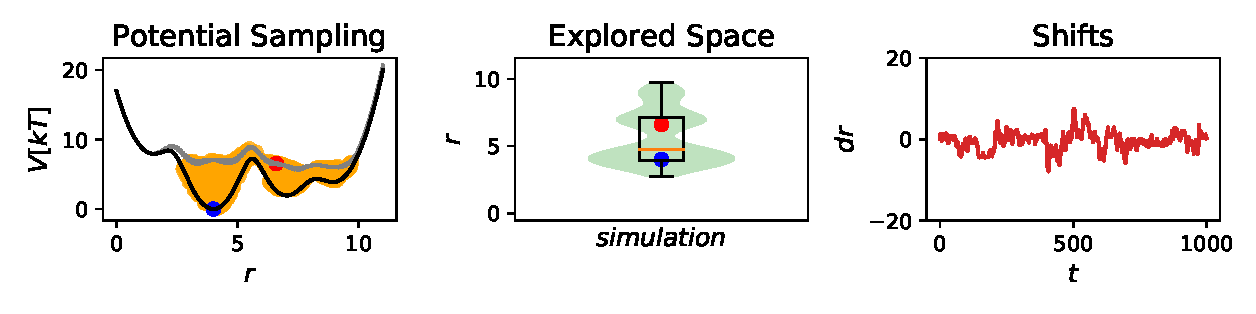
\includegraphics[width=0.85\linewidth]{fig/codeExamples/metaDynamics_simulation.pdf}
	\end{subfigure}
	\vspace{2.5mm}
	\begin{subfigure}{\textwidth}
		\caption{Example Source Code}
		\centering
		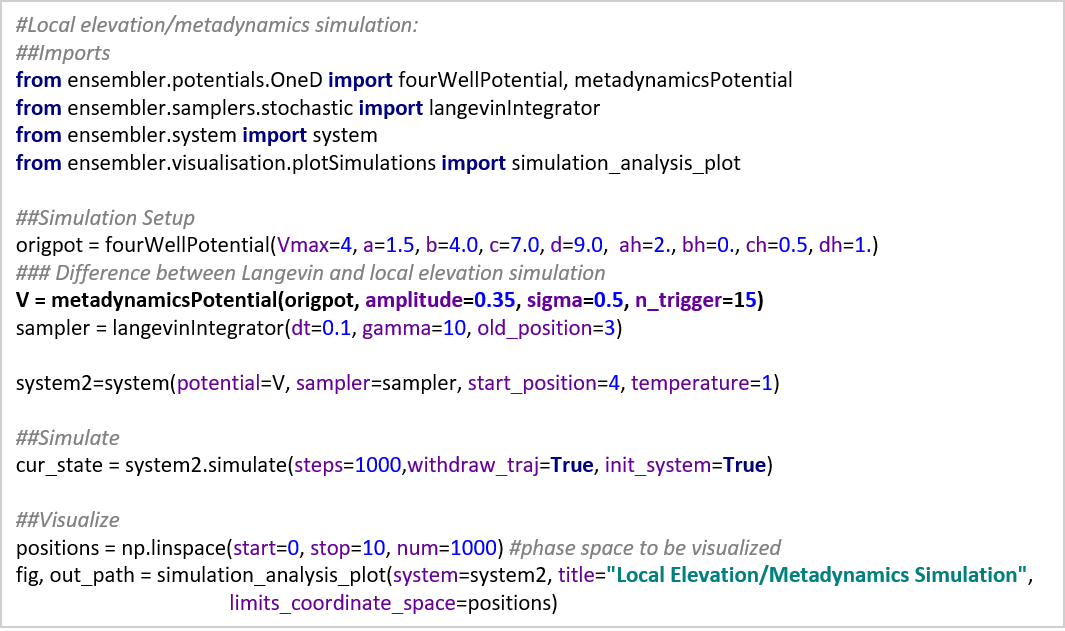
\includegraphics[width=0.85\linewidth]{fig/codeExamples/Simulation_code.png}
	\end{subfigure}
\caption{Langevin simulation of a four-well potential energy-function. Results when sampling (1000 steps) with the standard SD integrator (a) or with local elevation\cite{Huber1994}/metadynamics\cite{Laio2002} (b). The left panel shows the potential-energy surface (black), the sampled range (orange), as well as the start point (blue) and end point (red). The middle panel shows the sampled space as a violin/box plot with the start point (blue) and end point (red). The right panel shows the shift $\Delta r_t$ = $r_{t+1}$ - $r_t$ as a function of simulation time $t$.
	(c) Source code to perform the simulations. First, the four-well \textit{potential class} and the Langevin \textit{sampler class} are initiated. Next, they are wrapped by a \textit{system class}, which executes the simulation. Visualizations are generated with a built-in functions. Note that only one line has to be added to use the enhanced sampling technique (marked in bold).}
\label{fig:code_example_simulations}
\end{figure}


%-------------------------------------------------------------------------------------------------------------------------
\subsection{Free-Energy Calculation}
%-------------------------------------------------------------------------------------------------------------------------

Free-energy calculation is an important field in computational chemistry because free-energy differences govern the outcome of processes in nature, e.g. protein-ligand binding or polymer formation.\cite{Christ2009, Hansen2014, Cournia2020, Armacost2020} 
%
The calculation of alchemical free-energy differences with Ensembler is exemplified with a mutation of the equilibrium position of a one-dimensional harmonic oscillator (Figure \ref{fig:FE_sampling}a).
This mutation corresponds to a change of a covalent bond type at the terminus of a linear molecule and can be calculated analytically (Table \ref{tab:FE_results}).
In practical applications, however, it is usually not possible to calculate the free-energy difference analytically. In these cases, MD-based simulation techniques can be employed.
In the following, the sampling of the two end states of the model system and the results of the free-energy calculation with different methods are discussed. For more details, we refer to the Jupyter notebook in the Ensembler GitHub repository.

A simple free-energy method is to simulate one end state and estimate the free-energy difference with the Zwanzig equation.\cite{Zwanzig1954} The quality of the result depends on a sufficient phase-space overlap between the two end states.\cite{Konig2018}
Alternatively, one can simulate both end states separately and use BAR\cite{Bennett1976} (Figure \ref{fig:FE_sampling}a), yielding more converged results.\cite{Konig2018}
If the phase-space overlap between the two end states is not sufficient, more advanced sampling methods are necessary to obtain converged free-energy differences.
%
\begin{figure}[H]
	\centering
	\begin{subfigure}{.85\textwidth}
		\caption{}
		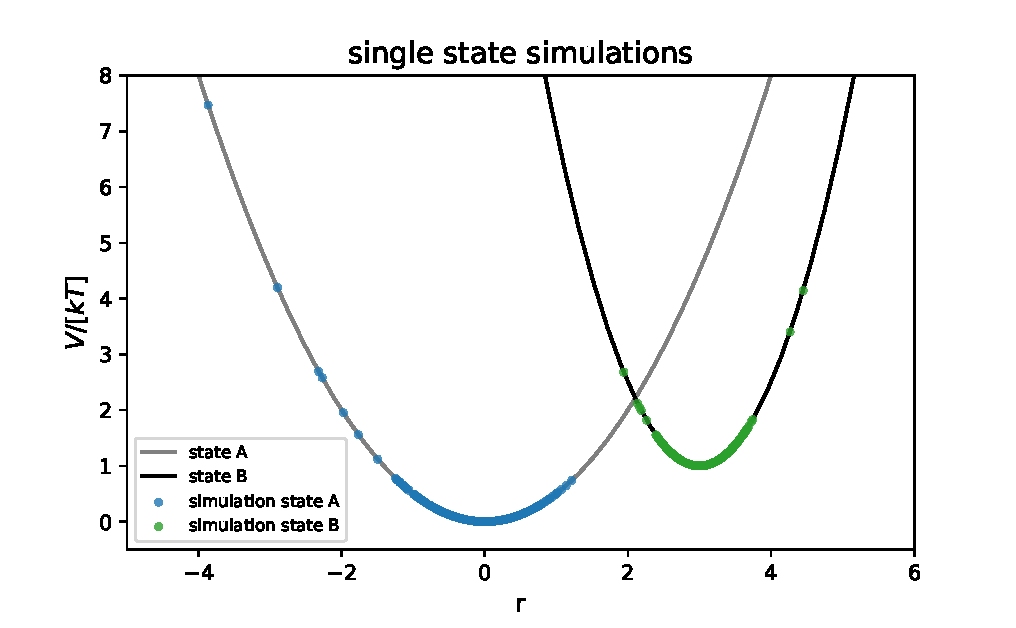
\includegraphics[width=\linewidth]{fig/FE_example/freeEnergyPertubation.pdf} 
	\end{subfigure}\\
	\begin{subfigure}{.85\textwidth}
		\caption{}
		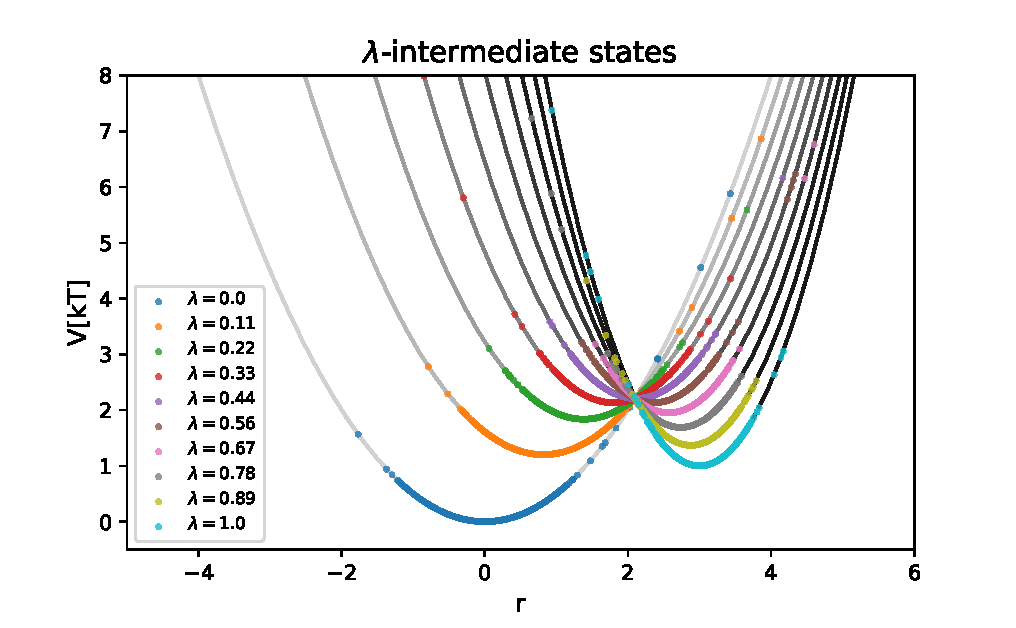
\includegraphics[width=\linewidth]{fig/FE_example/linear_coupled.pdf} 
	\end{subfigure}
	\caption{Illustration of different free-energy methods implemented in Ensembler (part I). (a) For FEP\cite{Zwanzig1954} and BAR\cite{Bennett1976}, the two end states (grey and black) are sampled separately (green and blue). (b) To increase the phase-space overlap, the two end states can be coupled as a linear combination of their Hamiltonians using a coupling parameter $\lambda$. This allows the generation of intermediate states (grey to black) and sampling of those (colored points).}
	\label{fig:FE_sampling}
\end{figure}
%
\begin{figure}[H]
	\centering
	\begin{subfigure}{.85\textwidth}
		\caption{}
		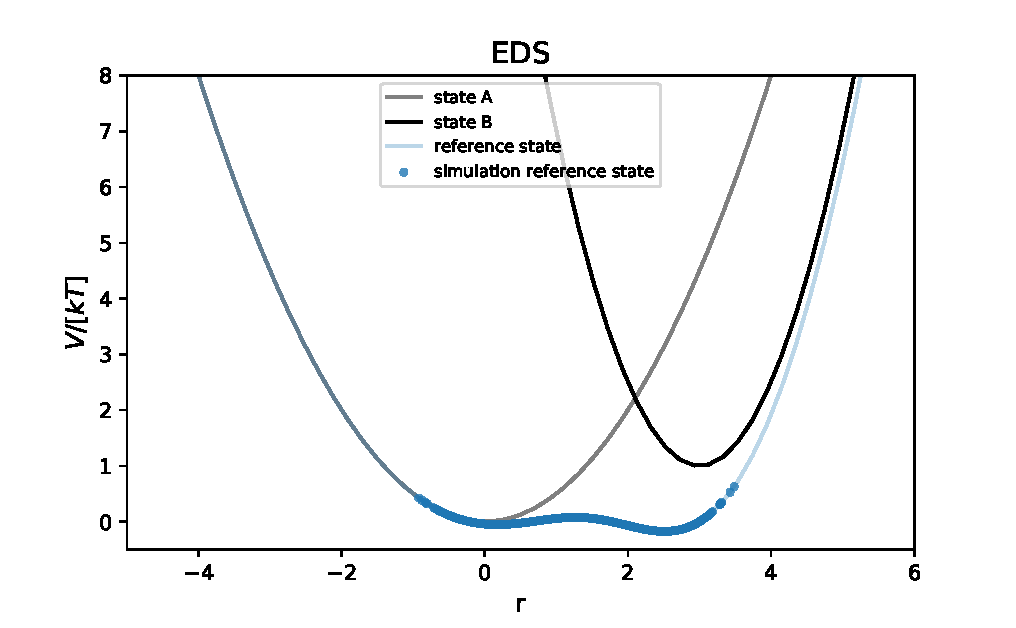
\includegraphics[width=\linewidth]{fig/FE_example/EDS_sampling.pdf} 
	\end{subfigure}\\
	\begin{subfigure}{.85\textwidth}
		\caption{}
		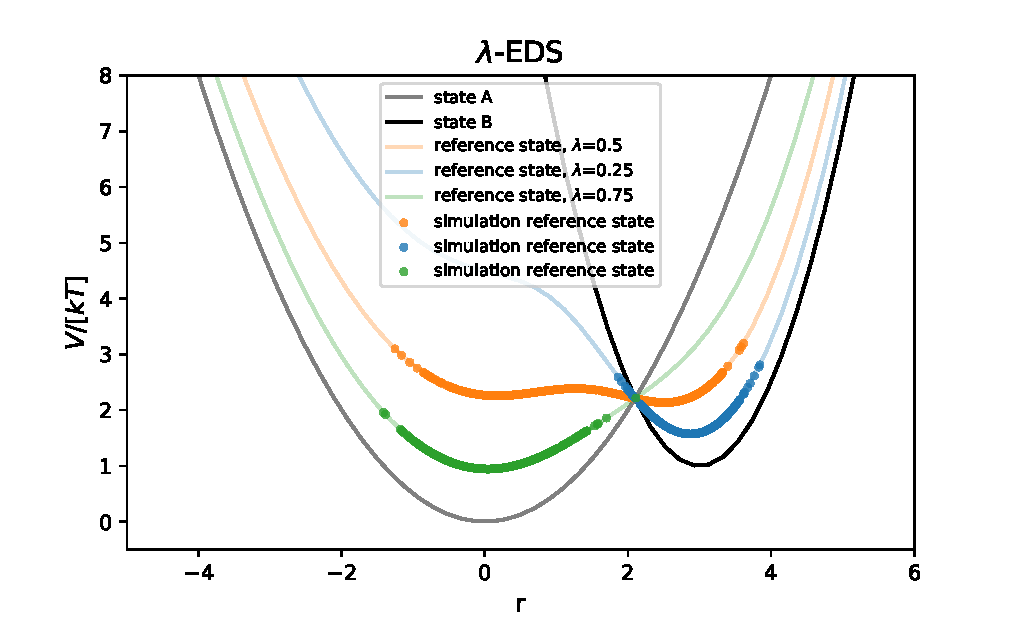
\includegraphics[width=\linewidth]{fig/FE_example/hlEDS_sampling.pdf} 
	\end{subfigure}
	\caption{Illustration of different free-energy methods implemented in Ensembler (part II). (a) An alternative method is EDS,\cite{Christ2007, Christ2008, Christ2009} where a reference-state Hamiltonian (blue line) is sampled (blue points), which envelopes the end states. By setting the reference-state parameters to $s$~=~0.3 and energy offsets~=~[0,0], all relevant phase-space regions can be sampled. (b) A recently developed approach called $\lambda$-EDS\cite{Koenig2020} introduces a $\lambda$-dependence in the EDS method (blue, orange and green line). Colored points indicate sampling. The reference-state parameters were set to $s$~=~0.3 and energy offsets~=~[0,0], and three different lambda values 0.25,0.5, 0.75 were chosen.}
	\label{fig:FE_samplingb}
\end{figure}
%%linear coupling
One possibility to increase the phase-space overlap is to generate intermediate states as a linear combination of the two end states $A$ and $B$ with the coupling parameter $\lambda$, i.e. $H(\lambda) = (1-\lambda) H_A + \lambda H_B$, such that $H(\lambda=0) = H_A$ and $H(\lambda=1) = H_B$.
The intermediate states are positioned at discrete $\lambda$-points between 0 and 1 (Figure \ref{fig:FE_sampling}b).\cite{Valleau1972, Straatsma1991} 
The free-energy difference can be estimated using FEP\cite{Zwanzig1954} or BAR\cite{Bennett1976} as the path over all intermediates, or with TI\cite{Kirkwood1935} as the integral along $\lambda$. 

%% EDS
Another elegant free-energy method is EDS,\cite{Christ2007, Christ2008} where a reference-state Hamiltonian $H_r$ is sampled. $H_r$ is constructed as a log-sum of the Hamiltonians of the two (or more) end states, guaranteeing the phase-space overlap of the reference state with all end states,
\begin{equation}
H_R = - \frac{1}{\beta s} \ln( e^{(- \beta s (H_A - E^R_A)}) +e^{(- \beta s (H_B - E^R_B)}),
\end{equation}
where $1/\beta=k_{B}T$, $k_B$ being the Boltzmann constant and $T$ the absolute temperature.
$H_R$ can be optimized for sampling using two kinds of parameters: The smoothing parameter $s$ lowers the energy barriers between the end states, whereas the energy offsets $E^R$ ensure equal weighting of all end states. In our example, both end states are sampled sufficiently during the EDS simulation with $s=0.3$ and the energy offsets $E^R=[0,0]$ (Figure \ref{fig:FE_sampling}c). Subsequently, the Zwanzig equation\cite{Zwanzig1954} is used to obtain the free-energy difference between the end states.\cite{Christ2007, Christ2008}
%hybrid coupling l-EDS
Recently, a hybrid form of EDS and $\lambda$-coupling was introduced, termed $\lambda$-EDS.\cite{Koenig2020} At $\lambda=0$ or $1$, the $H_R$ is equal to the Hamiltonians of the respective end states, while conventional EDS is recovered with $\lambda$=0.5 (except for an offset).\cite{Koenig2020}
$\lambda$-EDS allows for a $\lambda$-weighting of the exponential terms in the EDS equation. In the example in Figure \ref{fig:FE_sampling}d, the same reference-state parameters were used as before.

%final comparison
All free-energy calculations discussed above were performed with Ensembler for a total of 10'000 Monte Carlo (MC)\cite{Hastings1970} steps, and each simulation was repeated five times.
The simulation results listed in Table \ref{tab:FE_results} show that larger errors are obtained without intermediate states due to insufficient phase-space overlap.
Using ten $\lambda$–intermediate states together with TI gave the best result, however, this approach is also the computationally most expensive one (i.e. ten separate simulations). s
EDS and $\lambda$-EDS, on the other hand, yielded also good results, while requiring only one simulation (given a set of suitable reference-state parameters). 
We refer to the Jupyter notebook in the Ensembler GitHub repository for the source code, more detailed information on these methods as well as additional methods like conveyor-belt TI\cite{Hahn2019} and RE-EDS,\cite{Sidler2016, Sidler2017} which combine enhanced sampling and free-energy methods.
\begin{table}[ht]
	\centering
	\caption{Estimated free-energy difference for the model system shown in Figure \ref{fig:FE_sampling}. Sampling was performed with Monte Carlo (MC)\cite{Hastings1970} for 10'000 steps in each simulation. Each calculation was replicated five times and the averaged result is shown together with the standard deviation.
		The duration of the computations (without visualizations) was estimated directly in the Jupyter notebook and is given relative to the FEP simulation (absolute duration = 2.0 seconds). The performance was tested on a Lenovo Thinkpad T420s with an Intel i5-2520 ($2.5~\text{GHz}$) CPU and $8~\text{GB}$ RAM. The RAM usage for the full Jupyter notebook execution was in total $578~\text{MB}$.}
	\label{tab:FE_results}
	\resizebox{\columnwidth}{!}{%
		\begin{tabular}{l|r | c| r r}
			Method & Average $\Delta$F [$k_B T$] & Deviation from & \multicolumn{2}{c}{Speed (rel. to FEP)}\\
			&       & analytical result [$k_B T$] & Simulation & Analysis \\
			\hline
			\textit{analytical} & 1.275 & - & - & -  \\
			FEP\cite{Zwanzig1954} & $6.579 \pm  1.009$ & 5.305 & 1.0 & 0.1  \\
			BAR\cite{Bennett1976} & $2.437 \pm  0.500$ & 2.437 & 3.0 & 2.1 \\
			FEP 10-$\lambda$-points &  $1.406 \pm 0.431$ & 0.131 & 14.0 & 0.7 \\
			TI\cite{Kirkwood1935} 10-$\lambda$-points& $1.242 \pm 0.015$ & 0.033 & 14.0 & 0.04\\
			EDS\cite{Christ2007, Christ2008, Christ2009} &  $0.958 \pm 0.110$ & 0.317 & 2.4 &  0.2 \\
			$\lambda$-EDS\cite{Koenig2020} $\lambda=0.5$ & $ 0.987 \pm  0.111$ & 0.287 & 3.1 & 0.2\\
		\end{tabular}
	}
\end{table}
